\documentclass[conference]{IEEEtran}
\IEEEoverridecommandlockouts
\usepackage{cite}
\usepackage{amsmath,amssymb}
\usepackage{graphicx}
\usepackage{booktabs}
\usepackage{multirow}
\usepackage{xcolor}
\usepackage{tikz}
\usetikzlibrary{positioning,arrows.meta}
\usepackage{url}
\usepackage[hidelinks]{hyperref}
\graphicspath{{figures/}}

\begin{document}

\title{RedFlag Lens: Screening Indian Annual Reports\\for Credit Red Flags with Fine-Tuned Transformers}

\author{
\IEEEauthorblockN{Navnit Naman}
\IEEEauthorblockA{Enrollment No. 230085\\
Newton School of Technology\\
Rishihood University\\
Sonipat, Haryana, India}
\and
\IEEEauthorblockN{Kanhaiya Kumar}
\IEEEauthorblockA{Enrollment No. 230062\\
Newton School of Technology\\
Rishihood University\\
Sonipat, Haryana, India}
}

\maketitle

\begin{abstract}
Indian listed-company annual reports run to 200--400 pages, and the few sentences that matter to a lender, such as going-concern doubts, audit qualifications, loan defaults and insolvency proceedings, are scattered through them. We present RedFlag Lens, a system that reads an annual report PDF, scores every sentence for credit risk, assigns one of five risk categories, and returns a ranked, page-cited list of findings for a credit analyst. We built a corpus of 26 reports (10 from companies that later defaulted or collapsed, 16 healthy; 96,792 sentences) and split it by company to avoid year-over-year text leakage. With no time for human annotation, labels were produced by LLM annotators from different vendors under a written guide, with a third model breaking ties (Cohen's $\kappa$ 0.90 and 0.76 on the two halves of the test set). On a 600-sentence test set from five unseen companies, a three-seed ensemble of DeBERTa-v3-large trained with 600 extra non-risk examples reaches F1 0.86 (95\% CI 0.76--0.93) and recall 0.92, against 0.77 for fine-tuned FinBERT, 0.60 for TF-IDF, 0.56 for a zero-shot 7B LLM and 0.23 for keyword search. At report level, a pre-registered lexicon of severe early-warning signals applied to model output separates distressed from healthy reports with ROC-AUC 0.94 on eight reports, while the raw flag count scores 0.50. On two reports never used in any split, SpiceJet FY2023 (distressed) and Nestl\'e India FY2024 (healthy), the system finds 13.5 and 1.6 severe signs per 1,000 sentences. The system runs on a laptop CPU in about 2.5 minutes per report.
\end{abstract}

\begin{IEEEkeywords}
financial NLP, credit risk, annual reports, sentence classification, FinBERT, DeBERTa, LLM annotation, early warning signals
\end{IEEEkeywords}

\section{Introduction}
Before a bank or non-banking financial company (NBFC) lends to a company, or reviews an existing loan, a credit analyst reads its annual report. The warning signs a lender cares about are scattered across the directors' report, the management discussion, the auditor's report, the Companies (Auditor's Report) Order (CARO) annexure~\cite{caro2020} and the notes to accounts. They include going-concern doubts, qualified or adverse audit opinions, defaults and delays in repaying loans, insolvency petitions before the National Company Law Tribunal (NCLT), regulator penalties and disputed statutory dues. Such signals are often disclosed well before a collapse. For example, the FY2024 report of Gensol Engineering, which collapsed in 2025, contains a subsidiary auditor's adverse remark on page 187 and a going-concern note on page 184. Finding them by hand takes hours, and they are easy to miss.

Keyword search does not solve the problem, because the same phrases appear in boilerplate. Every auditor's report explains what it \emph{would} do if a material uncertainty about going concern existed, and CARO requires the auditor to state whether the company has defaulted, so most reports say ``the Company has not defaulted''. General-purpose large language models (LLMs) can read text, but sending borrower documents to a third-party API raises privacy and cost concerns, and generated quotations are not guaranteed to exist in the source.

We make four contributions:
\begin{enumerate}
\item A company-split corpus of 26 Indian annual reports with sentence-level risk, category and specificity labels, produced by cross-vendor LLM annotators with tie-breaking.
\item A comparison of keyword, TF-IDF, zero-shot LLM, FinBERT and DeBERTa-v3 classifiers on unseen companies, including augmentation with hard non-risk examples and seed ensembles.
\item A report-level evaluation (backtest) showing that \emph{severity}, not volume, of flagged text separates distressed from healthy companies.
\item A deployed system (FastAPI and Streamlit) with page-cited findings, failure handling, monitoring and an evidence-checked summary.
\end{enumerate}

\section{Related Work}
Dictionary methods dominate early financial text analysis; Loughran and McDonald~\cite{loughran2011} showed that general sentiment word lists misclassify financial text and built domain lists. Pre-trained transformers~\cite{devlin2019bert} improved financial sentiment classification; FinBERT~\cite{araci2019finbert} further pre-trains BERT on financial text and fine-tunes on the Financial PhraseBank~\cite{malo2014}. DeBERTa~\cite{he2021deberta} and DeBERTa-v3~\cite{he2023debertav3} improve on BERT with disentangled attention and ELECTRA-style pre-training. Averaging independently trained networks improves accuracy and calibration~\cite{lakshminarayanan2017}. LLMs have been shown to match or beat crowd workers on several annotation tasks~\cite{gilardi2023}, which motivates our use of LLM annotators, with agreement measured by Cohen's $\kappa$~\cite{cohen1960}. In India, the Reserve Bank of India's framework for loan frauds lists early-warning signals for lenders~\cite{rbi2015ews}; we use it to define our severity lexicon.

\section{Data}
\subsection{Corpus}
We downloaded 26 annual reports (8,303 pages) from the BSE archive: 10 from companies that later defaulted or collapsed (e.g., Jet Airways, Yes Bank, Reliance Communications, Gensol) and 16 from healthy companies (e.g., TCS, Maruti Suzuki, Titan, NTPC). Text was extracted page by page. Cleaning repaired the rupee glyph and ligatures, removed running headers and footers, split sentences with abbreviation-safe rules (``Rs.'', ``Ltd.'') and removed exact duplicates. This gave 96,792 sentences, each with its section and page. A fragment filter flags table rows, column headers and broken text (14,684 sentences, 15.2\%); on 300 pilot labels it catches 81\% of bad extractions and flags no risk sentence.

\subsection{Company-wise splits}
On average 27.7\% of a company's sentences repeat word for word from the previous year's report, so a sentence-level random split would leak. We split by company. Training uses 16 companies; validation uses RCOM, Titan and NTPC; the test set uses Jet Airways, Yes Bank, TCS, Maruti and Sun Pharma. Gensol FY2024 is held out from every split.

\begin{table}[t]
\caption{Company-wise splits and labelled sentences}
\label{tab:splits}
\centering
\setlength{\tabcolsep}{4pt}
\begin{tabular}{@{}llrr@{}}
\toprule
Split & Companies & Labelled & Risk \\
\midrule
Train & 16 companies & 1,590 & 211 \\
Validation & RCOM, Titan, NTPC & 260 & 30 \\
Test v1.1 & Jet, Yes Bank, TCS, Maruti, Sun Pharma & 600 & 37 \\
Held out & Gensol FY2024 & -- & -- \\
\bottomrule
\end{tabular}
\end{table}

\subsection{Labels}
Each sentence receives three labels under a written guide (v1.2): \emph{is\_risk} (would a credit analyst want this sentence on a ``things to check'' list), a \emph{category} (Financial, Legal, Regulatory, Operational, Business) with tie-breaking rules, and \emph{specificity} (a concrete event or finding versus generic wording). Nil confirmations (``no fraud was noticed''), auditor boilerplate and resolved litigation are non-risk.

No human annotation time was available, so labels come from LLM annotators. Training and validation sentences (1,590 and 260) were labelled by one Gemini model. Table~\ref{tab:splits} gives the sizes. The original 300 test sentences were labelled independently by Claude and by a second Gemini model, with a third Gemini model breaking the 4 disagreements; the training labeller never labelled test data. Because 16 risk sentences could not separate the models, we added 300 test sentences from the same companies (different sampling seed), labelled by Claude and Qwen2.5-32B-Instruct~\cite{qwen2024} served with vLLM~\cite{kwon2023vllm} at temperature 0 with JSON-constrained output; Llama-3.1-70B-Instruct~\cite{llama3} decided the 12 disagreements. The final test set v1.1 has 600 sentences, of which 37 are risks (Legal 16, Financial 12, Regulatory 7, Business 2). Agreement on \emph{is\_risk} is $\kappa=0.904$ on the first half and $\kappa=0.755$ on the second.

\section{Method}
\subsection{System pipeline}
Fig.~\ref{fig:pipeline} shows the pipeline. A PDF is validated, text is extracted with section and page, sentences are split, fragments are dropped, and each remaining sentence is scored by the classifier. Rules then remove nil statements, demote template and boilerplate text, and mark severe findings. Findings are ranked by (severe, specific, score), and a summary is generated and checked against the findings.

\begin{figure}[t]
\centering
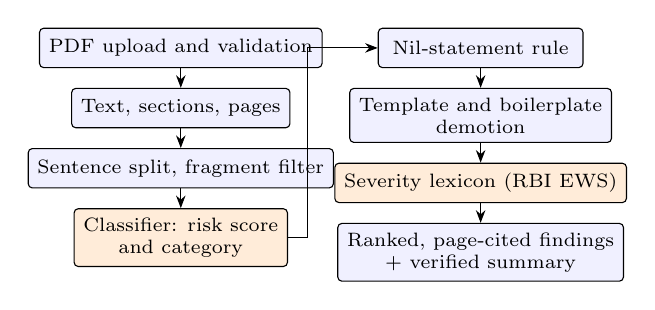
\begin{tikzpicture}[node distance=2.5mm, every node/.style={font=\scriptsize}, box/.style={draw, rounded corners=1.5pt, fill=blue!6, minimum width=26mm, minimum height=5mm, align=center}, >={Stealth[length=1.6mm]}]
\node[box] (a) {PDF upload and validation};
\node[box, below=of a] (b) {Text, sections, pages};
\node[box, below=of b] (c) {Sentence split, fragment filter};
\node[box, below=of c, fill=orange!15] (d) {Classifier: risk score\\and category};
\node[box, right=7mm of a] (e) {Nil-statement rule};
\node[box, below=of e] (f) {Template and boilerplate\\demotion};
\node[box, below=of f, fill=orange!15] (g) {Severity lexicon (RBI EWS)};
\node[box, below=of g] (h) {Ranked, page-cited findings\\+ verified summary};
\draw[->] (a)--(b); \draw[->] (b)--(c); \draw[->] (c)--(d);
\draw[->] (d.east) -- ++(2.5mm,0) |- (e.west);
\draw[->] (e)--(f); \draw[->] (f)--(g); \draw[->] (g)--(h);
\end{tikzpicture}
\caption{RedFlag Lens pipeline. The classifier scores every sentence; rules then filter and rank the findings.}
\label{fig:pipeline}
\end{figure}

\subsection{Baselines}
\emph{Keyword rules}: a 40-term red-flag regular expression. \emph{TF-IDF + logistic regression}~\cite{pedregosa2011}: word 1--2-grams and character 3--5-grams, class-balanced, with separate heads for risk, category and specificity. \emph{Zero-shot LLM}: Qwen2.5-7B-Instruct~\cite{qwen2024} given only the annotation guide, ten sentences per prompt, no training.

\subsection{Fine-tuned encoders}
We fine-tune FinBERT (\texttt{ProsusAI/finbert}) and DeBERTa-v3 base and large with the Transformers library~\cite{wolf2020}. Each model has one six-way softmax head over \{None, Financial, Legal, Regulatory, Operational, Business\}. The risk score of a sentence is $s = 1 - P(\text{None})$ and its category is the arg-max over the five risk classes. The section name is prepended to each sentence (e.g., ``[CARO] \ldots''), because the same words mean different things in the auditor's report and in the management discussion. Because only 13\% of training sentences are risks, we use class weights $w_c = (N / (K n_c))^{1/2}$. FinBERT trains for 4 epochs at learning rate $3\times10^{-5}$; DeBERTa for 5 epochs at $3\times10^{-5}$ (base) or $1\times10^{-5}$ (large) in bfloat16, with maximum length 128.

\subsection{Augmentation with hard negatives}
Most false alarms are sentences that contain risk words but are not risks. We add 600 real sentences from training companies as non-risk: 300 nil statements (``The Company has not defaulted in repayment of loans'') and 300 template or boilerplate sentences. Synthetic negation (rewriting risks as ``has not \ldots'') was tried and dropped, because many rewrites remained risky.

\subsection{Seed ensembles and model selection}
Each configuration (3 encoders $\times$ \{plain, augmented\}) is trained with 3 seeds, and the ensemble averages the class probabilities~\cite{lakshminarayanan2017}. The selection rule, fixed in advance, is the highest validation PR-AUC of the ensemble; the test set is used only to report. Training ran on rented RunPod GPUs (RTX 4090, L40S, A40).

\subsection{Report-level rules}
Three rules act on classifier output. (1) A \emph{nil rule} removes CARO-style negative confirmations. (2) \emph{Template and boilerplate demotion} moves questionnaire rows and any sentence that appears (after normalising digits and punctuation) in at least three training companies' reports (680 sentences) to a lower ``review'' tier. (3) A \emph{severity lexicon}, written from the RBI early-warning signals~\cite{rbi2015ews} \emph{before} the backtest was re-run, marks findings that mention going concern or material uncertainty, qualified, adverse or disclaimer opinions, default or delay in repayment, NPA classification, fraud or forensic audit, insolvency, NCLT or IBC proceedings, restructuring, rating downgrades, pledge invocation, auditor resignation or erosion of net worth. Findings with score $\ge 0.5$ that are not demoted form the default high-confidence list; a recall-oriented threshold tuned on validation (0.05) defines the review tier.

\section{Experiments and Results}
\subsection{Sentence-level results}
Table~\ref{tab:main} reports results on test set v1.1 at threshold 0.5. Confidence intervals are 95\% bootstrap intervals~\cite{efron1993} over sentences.

\begin{table*}[t]
\caption{Risk-sentence detection on test set v1.1 (600 sentences, 37 risk, 5 unseen companies)}
\label{tab:main}
\centering
\setlength{\tabcolsep}{8pt}
\begin{tabular}{@{}lccccc@{}}
\toprule
Model & P & R & F1 (95\% CI) & PR-AUC & Cat. F1 \\
\midrule
Keyword rules & 0.13 & 0.73 & 0.23 (0.15--0.30) & 0.11 & 0.18 \\
TF-IDF + LR & 0.52 & 0.70 & 0.60 (0.46--0.71) & 0.49 & 0.34 \\
Zero-shot Qwen2.5-7B & 0.45 & 0.73 & 0.56 (0.42--0.67) & 0.35 & 0.63 \\
FinBERT (app) & 0.70 & 0.84 & 0.77 (0.65--0.86) & 0.80 & \textbf{0.70} \\
FinBERT + aug, ens. & 0.73 & 0.81 & 0.77 (0.66--0.86) & 0.82 & 0.59 \\
DeBERTa-v3-base + aug, ens. & 0.71 & 0.81 & 0.76 (0.64--0.86) & 0.83 & 0.36 \\
DeBERTa-v3-large, ens. & 0.73 & 0.86 & 0.79 (0.68--0.88) & 0.89 & 0.50 \\
\textbf{DeBERTa-v3-large + aug, ens.} & \textbf{0.81} & \textbf{0.92} & \textbf{0.86 (0.76--0.93)} & \textbf{0.89} & 0.49 \\
\bottomrule
\end{tabular}
\end{table*}

Keyword search finds most risk sentences, but nine in ten of its flags are false alarms. The zero-shot 7B LLM is no better than TF-IDF. Fine-tuned encoders are clearly stronger, and the selected DeBERTa-v3-large + augmentation ensemble meets both targets set before the project (F1 $\ge$ 0.80, recall $\ge$ 0.85). Over three single seeds it scores F1 $0.84\pm0.03$, against $0.76\pm0.03$ without augmentation and $0.75\pm0.02$ for FinBERT, so augmentation mainly improves precision on template and nil text. On the 300 test sentences added last, on which no choice was ever made, the ensemble scores F1 0.93 (0.84--1.00) with recall 1.00. Category assignment is the weak point: the DeBERTa ensembles reach category macro-F1 0.49, against 0.70 for FinBERT, mostly from Legal/Regulatory confusion and the rare Business class.

\subsection{Error analysis and robustness}
On the original test set, most FinBERT false positives describe risk-management processes or generic exposure, and the two false negatives are short headings of contingent-liability tables. Replacing the rupee symbol with ``Rs.'' or ``INR'' changed one prediction; 4\% character-swap typos left recall unchanged and lowered precision. Negation is the clearest weakness: of 11 specific red flags rewritten as ``there were no instances where \ldots'', both FinBERT and TF-IDF still flagged 9; the nil rule removes them in the pipeline.

\subsection{Inference cost}
On a laptop CPU (Apple M2), FinBERT takes 45~ms per sentence, about 2.5 minutes for a full report including extraction, within the 3-minute target. A single DeBERTa-v3-large takes 341~ms per sentence on the CPU (about 16.5 minutes) but 1.4~ms on an RTX 4090 GPU (about 5 seconds per report). The app therefore uses FinBERT on a laptop and DeBERTa on a GPU server.

\subsection{Report-level backtest}
We ran the full pipeline, without an LLM, on eight complete reports: Gensol (held out), the four test companies with a clear outcome and the three validation companies. In a first run, healthy TCS and Maruti had \emph{more} high-confidence flags per 1,000 sentences than distressed Gensol and Yes Bank: large healthy companies disclose much routine litigation. After template demotion and the severity tier, Fig.~\ref{fig:backtest} and Table~\ref{tab:auc} show the result.

\begin{figure}[t]
\centering
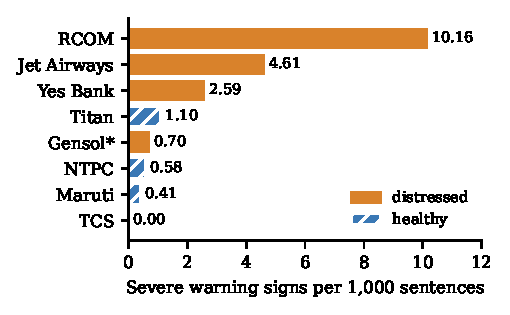
\includegraphics[width=\columnwidth]{backtest.pdf}
\caption{Severe warning signs per 1,000 sentences on eight full reports. *Gensol FY2024 was held out from every split.}
\label{fig:backtest}
\end{figure}

\begin{table}[t]
\caption{Separation of distressed from healthy reports (ROC-AUC)}
\label{tab:auc}
\centering
\begin{tabular}{@{}lcc@{}}
\toprule
Score per report & 8 reports & Gensol + test (5) \\
\midrule
High-confidence flags / 1k sentences & 0.50 & 0.33 \\
Specific flags / 1k sentences & 0.63 & -- \\
\textbf{Severe signs / 1k sentences} & \textbf{0.94} & \textbf{1.00} \\
\bottomrule
\end{tabular}
\end{table}

Counting flags measures how much a company discloses, not how distressed it is (AUC 0.50). Counting severe signs separates the groups with AUC 0.94; the only misordered pair is Gensol and Titan, whose three severe findings concern real credit exposure to IL\&FS. On Gensol the two severe findings are exactly the adverse remark (p.~187) and the going-concern note (p.~184). With 16 distressed--healthy pairs, this result is indicative rather than conclusive.

\subsection{Fresh test on unseen reports}
Finally, we ran the app model on two reports never used anywhere. SpiceJet FY2023 (217 pages, 2,515 sentences), an airline with negative net worth, produced 34 severe findings (13.52 per 1,000 sentences), more than any backtest report. They include the auditor's material uncertainty related to going concern, the basis for qualified opinion, ``unable to pay Rs.~750.00 million'' and lessors' Section~9 IBC petitions; about six are false alarms from a cargo business transfer ``as a going concern''. Nestl\'e India FY2024 (274 pages, 3,080 sentences) produced 5 severe findings (1.62 per 1,000), in the healthy range; all five are false alarms (an NCLT merger scheme, a standard revenue-fraud key audit matter and a business transfer agreement). Each report took about 2 to 2.5 minutes on the laptop.

\subsection{Targets set before building}
Table~\ref{tab:targets} compares the results with the targets fixed in the first milestone, before any model was built.

\begin{table}[t]
\caption{Targets fixed in advance and results}
\label{tab:targets}
\centering
\setlength{\tabcolsep}{3pt}
\begin{tabular}{@{}lll@{}}
\toprule
Metric & Target & Result \\
\midrule
Risk-sentence F1 (unseen companies) & $\ge 0.80$ & 0.86 (DeBERTa ens.) \\
Recall on risk sentences & $\ge 0.85$ & 0.92 (DeBERTa ens.) \\
Category macro-F1 & $\ge 0.70$ & 0.70 (FinBERT) \\
Time per report, laptop CPU & $\le 3$ min & $\sim$2.5 min (FinBERT) \\
Distressed vs healthy ROC-AUC & $\ge 0.75$ & 0.94 (8 reports) \\
Summary claims supported & $\ge 95\%$ & not measured \\
\bottomrule
\end{tabular}
\end{table}

\section{Deployment}
The pipeline is served by a FastAPI service (\texttt{POST /analyze}, \texttt{POST /feedback}, \texttt{GET /health}) and a Streamlit dashboard that shows severe signs first, headline counts, a summary, a filterable findings table, the cited page with the sentence highlighted, and thumbs-up/down feedback. A Dockerfile builds both. The summary is written by an LLM that must cite finding identifiers; a verifier drops claims that cite missing identifiers or rupee amounts not present in the cited sentences. If the LLM is unavailable, a template summary is built from the findings.

Invalid, password-protected or scanned PDFs, and files over 700 pages or 60~MB, return explicit errors. Each report writes one monitoring record with page and sentence counts, findings per category, the share of low-confidence scores (0.35--0.65), verifier rejections and time per stage. Alerts fire if the finding rate or the low-confidence share moves more than $2\times$ from the test baseline, a sign of a new report format or sector, or if LLM errors exceed 10\%. Reports are public statutory filings and the tool profiles companies, not individuals; the classifier runs locally.

\section{Limitations}
(1) Labels are LLM-generated; errors shared by all annotators would not show up, and the second half of the test set has lower agreement ($\kappa=0.76$). (2) The test set is still modest (37 risks; Business has 2), and the backtest uses eight reports. (3) Category assignment by the best detector is weak (macro-F1 0.49). (4) The models react to risk words in negated sentences; a rule covers the common patterns. (5) The severity lexicon confuses NCLT merger schemes and business transfers ``as a going concern'' with distress, and bank reports use ``fraud'' and ``NPA'' routinely. (6) Rows of contingent-liability tables are excluded as fragments. (7) We compared against one open 7B LLM only; larger hosted LLMs were not evaluated. (8) The LLM summary verifier was not run on real LLM output because API credit ran out.

\section{Conclusion and Future Work}
RedFlag Lens reads an entire annual report and puts the sentences a lender should check at the top, each with its page. A DeBERTa-v3-large ensemble trained with hard non-risk examples detects risk sentences in unseen companies with F1 0.86 and recall 0.92, and the rate of severe early-warning signs separates distressed from healthy reports (ROC-AUC 0.94 on eight reports; 13.5 against 1.6 per 1,000 sentences on two fresh reports). Future work: human labels for the test set, a backtest on 30 or more reports across sectors, a hybrid in which DeBERTa detects and FinBERT categorises, a context-aware severity model, table extraction for contingent liabilities, year-over-year differencing, and comparison with larger LLMs.

\section*{Code and Data Availability}
Code, evaluation outputs and the experiment log are available at \url{https://github.com/naman394/redflag-lens}. Trained weights are kept outside the repository because of their size.

\begin{thebibliography}{00}
\bibitem{caro2020} Ministry of Corporate Affairs, Government of India, ``Companies (Auditor's Report) Order, 2020,'' Feb. 2020.
\bibitem{loughran2011} T. Loughran and B. McDonald, ``When is a liability not a liability? Textual analysis, dictionaries, and 10-Ks,'' \emph{J. Finance}, vol. 66, no. 1, pp. 35--65, 2011.
\bibitem{devlin2019bert} J. Devlin, M.-W. Chang, K. Lee, and K. Toutanova, ``BERT: Pre-training of deep bidirectional transformers for language understanding,'' in \emph{Proc. NAACL-HLT}, 2019, pp. 4171--4186.
\bibitem{araci2019finbert} D. Araci, ``FinBERT: Financial sentiment analysis with pre-trained language models,'' arXiv:1908.10063, 2019.
\bibitem{malo2014} P. Malo, A. Sinha, P. Korhonen, J. Wallenius, and P. Takala, ``Good debt or bad debt: Detecting semantic orientations in economic texts,'' \emph{J. Assoc. Inf. Sci. Technol.}, vol. 65, no. 4, pp. 782--796, 2014.
\bibitem{he2021deberta} P. He, X. Liu, J. Gao, and W. Chen, ``DeBERTa: Decoding-enhanced BERT with disentangled attention,'' in \emph{Proc. ICLR}, 2021.
\bibitem{he2023debertav3} P. He, J. Gao, and W. Chen, ``DeBERTaV3: Improving DeBERTa using ELECTRA-style pre-training with gradient-disentangled embedding sharing,'' in \emph{Proc. ICLR}, 2023.
\bibitem{lakshminarayanan2017} B. Lakshminarayanan, A. Pritzel, and C. Blundell, ``Simple and scalable predictive uncertainty estimation using deep ensembles,'' in \emph{Proc. NeurIPS}, 2017.
\bibitem{gilardi2023} F. Gilardi, M. Alizadeh, and M. Kubli, ``ChatGPT outperforms crowd workers for text-annotation tasks,'' \emph{Proc. Natl. Acad. Sci.}, vol. 120, no. 30, 2023.
\bibitem{cohen1960} J. Cohen, ``A coefficient of agreement for nominal scales,'' \emph{Educ. Psychol. Meas.}, vol. 20, no. 1, pp. 37--46, 1960.
\bibitem{rbi2015ews} Reserve Bank of India, ``Framework for dealing with loan frauds,'' RBI circular, May 2015.
\bibitem{qwen2024} Qwen Team, ``Qwen2.5 technical report,'' arXiv:2412.15115, 2024.
\bibitem{kwon2023vllm} W. Kwon \emph{et al.}, ``Efficient memory management for large language model serving with PagedAttention,'' in \emph{Proc. ACM SOSP}, 2023.
\bibitem{llama3} A. Grattafiori \emph{et al.}, ``The Llama 3 herd of models,'' arXiv:2407.21783, 2024.
\bibitem{pedregosa2011} F. Pedregosa \emph{et al.}, ``Scikit-learn: Machine learning in Python,'' \emph{J. Mach. Learn. Res.}, vol. 12, pp. 2825--2830, 2011.
\bibitem{wolf2020} T. Wolf \emph{et al.}, ``Transformers: State-of-the-art natural language processing,'' in \emph{Proc. EMNLP: System Demonstrations}, 2020, pp. 38--45.
\bibitem{efron1993} B. Efron and R. J. Tibshirani, \emph{An Introduction to the Bootstrap}. New York, NY, USA: Chapman \& Hall, 1993.
\end{thebibliography}

\end{document}
